\documentclass[authoryear]{elsarticle}
\usepackage{amsmath}
\usepackage{graphicx,psfrag,epsf,comment}
\usepackage{enumerate}
\usepackage{url} % not crucial - just used below for the URL 
\bibliographystyle{chicago}
\usepackage{threeparttable}

\newcommand{\logit}{\mathrm{logit}}
\newcommand{\I}{\mathrm{I}}
\newcommand{\E}{\mathrm{E}}
\newcommand{\p}{\mathrm{P}}
\newcommand{\e}{\mathrm{e}}
\renewcommand{\o}{\omega}
\newcommand{\vecm}{\mathrm{vec}}
\newcommand{\kp}{\otimes}
\newcommand{\diag}{\mathrm{diag}}
\newcommand{\cov}{\mathrm{cov}}
\newcommand{\eps}{\epsilon}
\newcommand{\ep}{\varepsilon}
\newcommand{\obdots}{\ddots}    % change this later
\newcommand{\Ex}{{\cal E}}
\newcommand{\Ax}{{\mathrm{A}}}
\newcommand{\Exd}{\Ex_d}
\newcommand{\Es}{\Ex}
\newcommand{\rat}{{\frac{c_{ij}}{c_{i,j-1}}}}
\newcommand{\rmu}{m}
\newcommand{\rsig}{  r}
\newcommand{\fd}{\mu}
\newcommand{\tr}{\mathrm{tr}}
\newcommand{\cor}{\mathrm{cor}}
\newcommand{\bx}[1]{\ensuremath{\overline{#1}|}}
\newcommand{\an}[1]{\ensuremath{a_{\bx{#1}}}}

\newcommand{\bi}{\begin{itemize}}
\newcommand{\ei}{\end{itemize}}

\renewcommand{\i}{\item}
\newcommand{\sr}{\ensuremath{\mathrm{SRISK}}}
\newcommand{\br}{\ensuremath{\mathrm{BRISK}}}
\newcommand{\pr}{\ensuremath{\mathrm{PRISK}}}
\newcommand{\cs}{\ensuremath{\mathrm{CS}}}
\newcommand{\cri}{\ensuremath{\mathrm{Crisis}}}
\newcommand{\var}{\ensuremath{\mathrm{VaR}}}
\newcommand{\covar}{\ensuremath{\mathrm{CoVaR}}}
\newcommand{\med}{\ensuremath{\mathrm{m}}}
\newcommand{\de}{\mathrm{d}}
\renewcommand{\v}{\ensuremath{\mathrm{v}_q}}
\newcommand{\m}{\ensuremath{\mathrm{m}}}
\newcommand{\tvar}{\ensuremath{\mathrm{TVaR}}}
\renewcommand{\c}{\ensuremath{\mathrm{CoVaR_q}}}
\renewcommand{\v}{\ensuremath{\mathrm{VaR}_q}}

\newcommand{\eref}[1]{(\ref{#1})}
\newcommand{\fref}[1]{Figure \ref{#1}}
\newcommand{\sref}[1]{Section \ref{#1}}
\newcommand{\tref}[1]{Table \ref{#1}}
\newcommand{\aref}[1]{Appendix \ref{#1}}

\newcommand{\cq}{\ , \qquad}
\renewcommand{\P}{\mathrm{P}}
\newcommand{\Q}{\mathrm{Q}}

\newcommand{\Vx}{{\cal V}}
\newcommand{\be}[1]{\begin{equation}\label{#1}}
\newcommand{\ee}{\end{equation}}



\begin{document}

\title{An early warning system for monitoring  stress in the financial system}
%\author[acst]{Piet de Jong\corref{cor1}\footnote{The authors gratefully acknowledge CIFR, the Centre of International Financial Regulation for financial support and other assistance}}
%\ead{piet.dejong@mq.edu.au}
%\author[acst]{Geoffrey Loudon}
%\author[acst]{Weihao Choo}
%\address[acst]{Department of Applied Finance and Actuarial Studies Macquarie University, NSW 2109, Australia.}
%\cortext[cor1]{Corresponding author}


\begin{abstract}
SRISK methodology recently proposed in the literature is refined and extended using a formalised stress testing framework.  The framework defines two types of risk:  baseline risk and the stress risk, corresponding to ordinary and ``stressed" expectation, respectively, given a time series model and past observations.   Stressed expectation is expectation computed  under a hypothetical  stress, modelled with a stress function and scenarios.   Stress functions are chosen by the practitioner and  exaggerate the probability undesirable  outcomes.    Properties and characterisations of stress and stress related quantities are displayed and explored.  Systemic stress is defined in terms of stresses   impacting groups of firms or financial entities.    Application is made to the study of the stability of Australian banks using daily time series data.
\end{abstract}

\date{}
\maketitle
\noindent
{\it Keywords:}  Capital shortfall, baseline risk, stress testing,  stressed expectation, stress diversification.


\newpage

\section{Introduction}\label{intro}
Monitoring stresses and systemic risk in the financial system is a key function of macro--prudential regulation. Central banks and other financial regulatory bodies such as the US Financial Stability Oversight Council, the European Systemic Risk Board and the Australian Prudential Regulation Authority (APRA) are concerned with developing and applying early warning quantitative  measures  to warn of potential episodes of heightened systemic risk. 

Systemic risk has many dimensions. For example, in their influential review paper, \cite{Bisias2012} present a taxonomy of six categories of systemic risk comprising 31 quantitative risk measures. While attempts to gain consensus on a theoretical definition have proved elusive, several empirical measures of systemic risk have been developed and applied with  success.  An important example is the SRISK measure due to \cite{brownlees2015} -- an index that measures the expected capital shortfall of a financial institution conditional on a large and lengthy decline in equity markets. \cite{brownlees2015} show that their SRISK based measures are able to identify systemically important financial firms and are informative about the impact of financial crises on future macro-economic conditions. 

This paper refines and extends the SRISK model of \cite{brownlees2015} in  key ways. First SRISK is formalised  as a put on the expected shortfall with the ordinary expectation defined as the baseline risk (\br) associated with the put.   Using a stress function  the so--called stressed expectation is used to measure the impact of stress.   Stressed expectation can be similar to the \cite{brownlees2015} conditional expectation given  a severe market downturn.  However our generalised methodology  permits a more flexible definition of stress and a wider class of ``stressors" including stress defined in terms of  a number of extreme outcomes.  The difference between the stressed and ordinary expectation is defined as the stress risk associated, called \pr\ where P stand for psi,  the function $\psi$ modelling the stress. 

\br\  and \pr\  capture different aspects of stress on a firm. \br\  is a function of existing volatility and leverage. As these factors increase, \br\  rises and this makes the firm more susceptible to \pr, regardless of the stress event itself.   Properties of \pr\  are explored.
   
\cite{brownlees2015} define stress by conditioning on an absolute cutoff of arbitrary size and length. With time dependent volatility or uncertainty, absolute cutoffs  are less meaningful and our development suggests  it is  useful to specify conditional behaviour in percentile terms relative to current market conditions. This yields a sharper focus on the incremental impact of further stress and permits a more incisive view of the  implications from SRISK numbers. These extensions provide additional insights into the sources and economic nature of for example systemic risk. The measures provide potentially new and improved ways of anticipating episodes of heightened systemic risk. Their practical use can be expected to help regulators monitor risk including systemic risk and contagion in timely fashion,   facilitating remedial action where necessary.

While our measures are designed for use in all financial systems, it is of particular interest to test them using the Australian setting for at least two reasons. First, the Australian financial system is dominated by only four banks. In Australia there are four major banks that hold 78\% of the total assets of all Authorised Deposit-taking Institutions in  Australia.\footnote{Based on balances at 31 December 2014 disclosed in APRA's Quarterly Authorised Deposit-taking Institution (ADI) Performance Report for March 2015.} It is therefore obvious that the four majors are systemically important and the remaining ADIs are not so unless stress in one of these minors somehow creates financial contagion to the majors, in an unforeseeable way. Second, the Australian banking system proved to be resilient through the recent global financial crisis (GFC), implying that systemic risk did not reach the extreme levels experienced by other countries where bank failures occurred. Both these features of the Australian system suggest that it may be difficult to find useful additional information about systemic risk by refining quantitative measures like SRISK. Since we are able to show that our measures are informative about systemic risk in Australia, we conjecture that they will provide additional insights elsewhere.  

The nature and usefulness of our measures are demonstrated using publicly available daily financial data for the eight Australian banks detailed in \tref{eightbanks} spanning the period from  3 April 2000 through to 1 December 2014.  The data is described in detail in \aref{data}.  Prices, adjusted for dividends are plotted in \fref{prices}.  Prices are combined with number of shares to derive total equity. Total debt for each firm is also collected from annual accounting reports. 

Remaining sections are structured as follows. Section \ref{litrev} briefly discusses related literature. Section \ref{capshort} defines current and future  capital shortfall similarly as \cite{brownlees2015} under a simple Basel II regulatory framework. The definition of systemic risk used by \cite{brownlees2015} is discussed, refined and improved in \sref{srisk}. Applications to Australian bank data are discussed in \sref{simulate} and \sref{simulate1}. Section \ref{aggregate}  discusses the aggregation of  stresses across firms with and without allowance for merging or diversification. Section \ref{monitoring} displays stress calculations as they would proceed in real time.   Section \ref{riskmethod} offers an alternative modelling approach, based on assets.  Section \ref{conclude} concludes.

\begin{table}[htbp]
\label{banks}\caption{Major and minor Australian banks}\label{eightbanks}
\begin{center}
\begin{tabular}{l|l|l|l}
\hline
 \multicolumn{2}{c|}{major}& \multicolumn{2}{c}{minor}\\
 \hline
CBA & Commonwealth Bank  & MQG & Macquarie \\
ANZ & Australia \& New Zealand  & BOQ & Bank of Queensland\\
NAB & National Australia  & BEN & Bendigo and Adelaide \\
WBC & Westpac & ABA& Auswide \\
\hline
\end{tabular}
\end{center}
\end{table}%


\begin{figure}[htbp]
\label{prices}
\begin{center}
 \begin{tabular}{cc}
      \resizebox{55mm}{!}{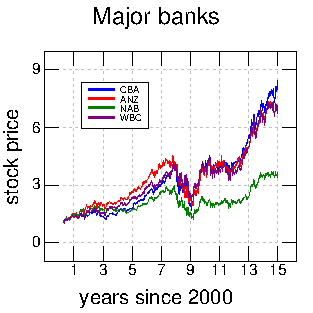
\includegraphics{figures/fig1a.pdf}} &
      \resizebox{55mm}{!}{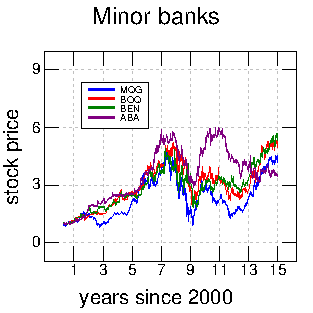
\includegraphics{figures/fig1b.pdf}}\\
    \end{tabular}
\caption{Daily stock  prices of four major (left panel) and four minor (right panel) Australian banks 2000--2014.  Price series normalised to start at 1.}
\end{center}
\end{figure}


\section{Literature review}\label{litrev}
Many papers in the finance and economics literature are devoted to the development and application of a variety of quantitative measures of systemic risk or financial stress. \cite{Bisias2012} provide an instructive and qualitative survey of numerous measures in use. \cite{Giglio2015} supply empirical evidence on the ability of many of these measures, both individually and collectively, to provide early warning signals of deterioration in macro-economic conditions. In this section, we provide a selective overview of those measures most closely related to SRISK and its relevance for assessing systemic risk in the financial sector. 

The genesis of SRISK lies in a series of papers including \cite{acharya2012aer}, \cite{acharya2012wp} and \cite{brownlees2010volatility}. In these papers, SRISK is defined as the expected capital shortfall of a financial firm, conditional on a crisis. A crisis is deemed to occur whenever a relevant market index suffers a significant decline over a chosen horizon. SRISK measures require an estimate of the long run marginal expected shortfall (LRMES) typically obtained by simulation methods.

\cite{brownlees2015}  develop empirical methodology to construct SRISK measures. SRISK depends on the firm's size, leverage and its LRMES. The LRMES is obtained by assuming a dynamic process for the joint distribution of firm and market returns. \cite{brownlees2015} use  the standard GARCH-DCC model of \cite{engle2002dynamic} with threshold ARCH volatilities on the basis that this represents a good trade-off between model complexity and prediction accuracy. The LRMES is computed as the Monte Carlo average of simulated multi-period returns,  conditional on the return being worse than the cut-off level chosen to identify a financial crisis. Using a sample of large US financial firms,  \cite{brownlees2015} show the practical usefulness of their measure in three ways: (i) SRISK rankings identify systemically risky US banks during the GFC; (ii) pre-crisis SRISK helps predict capital injections by the Fed Reserve; (iii) aggregate SRISK provides early warning of declines in industrial production and higher unemployment.
     
\cite{Engle2015} extend the model in \cite{brownlees2015} to incorporate global, country and industry effects. This extended model makes  use of the \citep{Engle2014dcb} dynamic conditional beta model. Their empirical methods are able to provide information about the relative systemic importance of industry type and country identity. For instance, they find  that systemic risk in Europe during the GFC was predominantly due to banks while France and the UK recorded the largest country-level SRISK numbers. 

\cite{adrian2011covar} propose an alternative measure of systemic risk  emphasising the co--dependence of financial firms and the importance of risk spillovers within the financial sector. They introduce CoVaR$_i$ which computes the Value--at--Risk (VaR) of the entire financial system, conditional on institution $i$ being in distress. Distress is defined as the state where the institution is exactly at its VaR level. \cite{Girardi2013} improve CoVaR by conditioning on the institution being at most at its VaR. This generalisation is useful as it takes into account the severity of tail losses and facilitates back--testing of CoVaR. 

\cite{acharya2012aer} relate SRISK and CoVaR and demonstrate that assuming the joint distribution of returns is conditionally normal, SRISK is a more complete measure. \cite{Benoit2013} show how several popular systemic risk measures including MES, CoVaR and SRISK are different transformations of market risk measures and derive those conditions under which they provide similar rankings of systemically important financial institutions.

Empirical estimates of SRISK  requires a model for the joint distribution of returns of individual firms and the market. Many of these papers use \cite{engle2002dynamic}'s GARCH--DCC model aiming to capture the time-varying dynamics of the return (co)variances in a feasible manner. While we also use this model in our empirical analysis, we emphasize that our approach can utilise any appropriate model for simulating the joint distribution of firm and market returns going forward. 

\section{Capital shortfall, leverage and future shortfall}\label{capshort}

If $d$ and $w$ are the debt and equity, respectively, of a particular  firm at a particular point of time, and $k$ is the prudential requirement,  then  as defined \cite{brownlees2015}, the  capital shortfall at that time is
\be{shortfall}
k (d+w)-w = k d\left(1-\frac{1-k}{kL}\right)=kd\left(1-\e^{-\ell}\right)
\ ,
\ee
where
$$
L\equiv\frac{d}{w}\cq \ell\equiv\ln\left(\frac{kL}{1-k}\right) = \logit(k) + \ln(L) \ .
$$
The quantity $\ell$ is called the adjusted log--leverage of firm  and $\ell>0$ implies, for the given $k$, capital shortfall is positive. The parameter $k$ is the proportion of assets $d+w$ excluded from capital calculations, and higher $ k$ leads to higher capital shortfall.   

The $\logit(k)$ enters $\ell$ as an additive constant and has  minor role in the technical development and can be varied to test for senstivity etc.  Assume\footnote{See for example \cite{brownlees2015}.} $k=0.08$ as under Basel II implying $\logit( k)=-2.44$ and the adjusted log--leverage $\ell$ is the actual log--leverage minus 2.44.  At this $k$, if $S>0$ there is positive capital shortfall and  the firm or financial institution is said be in ``Basel default" or a ``Basel breach" has occurred.   If $S<0$ there is capital surplus and  the firm is said to be ``Basel compliant."

The definition of capital shortfall in \eref{shortfall} is restrictive if not simplistic.   It is used here to conform to the previous literature and provide an easily accessible  platform to the key results of this paper,  without becoming entangled in precise and perhaps more realistic definitions of shortfall.   \sref{riskmethod} deals with a more realistic and intricate definition.  

\fref{Bloglev} displays adjusted log--leverages $\ell$ with $ k=0.08$ for the four major and four minor Australian banks listed in \tref{banks} on the first trading day of each month from January 2003  through to December 2014.  Note most banks are Basel compliant up to about 2008, entering into Basel breaches from 2009 as a result of the GFC. Prolonged Basel breaches are experienced for particular banks, notably NAB.


\begin{figure}[htbp]
\begin{center}
 \begin{tabular}{cc}
      \resizebox{55mm}{!}{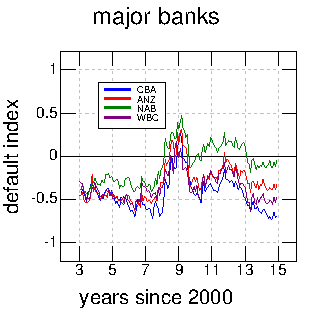
\includegraphics{figures/fig2a.pdf}} &
      \resizebox{55mm}{!}{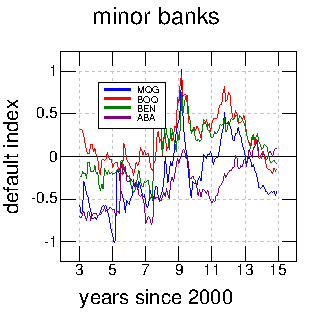
\includegraphics{figures/fig2b.pdf}}\\
    \end{tabular}
\caption{Adjusted log--leverages for four major (left panel) and four minor (right panel) Australian banks from the beginning of 2003 through to end of 2014.  All banks contravene the threshold (corresponding to the zero horizontal) around the start of 2009.}\label{Bloglev}
\end{center}
\end{figure}


Financial institutions and regulators are concerned with future shortfall.   Future shortfall depends on the future return on equity.   If $r$ is the future return on equity over say a month then the  equity in one month's time is $w\e^r$ and future shortfall is
\be{fshortfall}
  S\equiv k d\left(1-\frac{1-k}{kL\e^{-r}}\right) = kd(1-\e^{r-\ell})\ .
\ee
This assumes debt $d$ stays constant over the month.   The future return $r$ is unknown but its probability distribution may be modelled and relatively well understood.

The  future capital shortfall is $S^+$, the positive part of $S$:
\be{bs}
S^+ = kd (1-\e^{r-\ell})^+=\left\{\begin{array}{lr} 0\ , & r\ge \ell\ ,\\ kd (1-\e^{r-\ell})\ , & r<\ell\ .\end{array}\right.
\ee
Thus $S^+$ is $kd$ times a put on the return $\e^{r-\ell}$ with strike 1.  Default put options similar to \eref{bs} have been discussed in the insurance literature as critical to an evaluation of a firm:  see for
example \citet{merton1977analytic}, \citet{doherty1986price}, \citet{cummins1988risk}, \citet{myers2001capital} and \citet{sherris2006solvency}.

To appreciate the behaviour of $S$ and $S^+$, \fref{simulation}   displays two snapshot outputs from projections generated as described  in \aref{garchdcc}:  6000  simulated one month ahead projected returns for  CBA and the wider market, on  two dates: the first trading day in January 2009 and the first trading day in December 2014.  The CBA returns are used to calculate the future shortfall per units $kd$ as in \eref{fshortfall}.  Both panels use the same horizontal and vertical scales.   Based on the available data at those two points in  time, policy makers and regulators faced entirely different projections.   The scatter of dots are the forward simulations.  Note there is no hindsight bias as the model at each time point is based on the available data to that point in time.     In the left panel $S>0$ for most scenarios.    In the right panel $S<0$ for any conceivable market scenario.

 The black dots in each panel indicate the actual outcome after one month.    In the left panel the outcome is a decline in both  the market and CBA stock price.    In the right panel there is slight decline in the stock price, and a more substantial market downturn.    Thus at the beginning of January  2009 the one month forward projection for  CBA was far from compliance, while in December 2014 the one month forward projection is of complete compliance.

The two panels  display very different volatility and slopes. In January 2009 both CBA and the market return distributions are highly volatile and correlated. The correlation remains strong in December 2014 but with less return volatility.  Subsequent sections of this paper use time series of these  snapshots  to compute cross sectional and longitudinal baseline and systemic stresses.

\begin{figure}[htbp]
\begin{center}
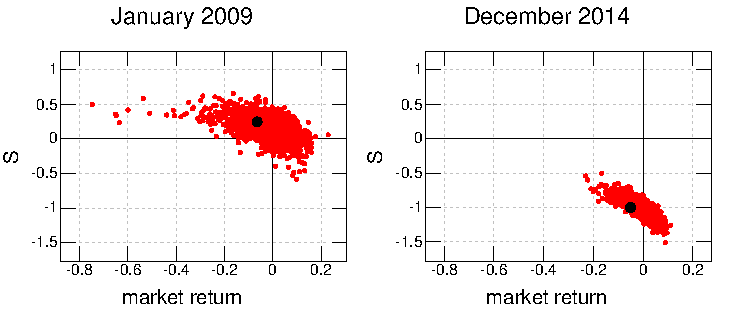
\includegraphics[width=12cm]{figures/figCBA.pdf}
\caption{Forecast bivariate distribution of future shortfall $S$ per unit $kd$  for CBA (vertical axis) and market rate of return (horizontal axis) at start of January 2009 (left panel)  and December 2014 (right panel). Note scales in both panels are the same, the relatively large volatility in the left panel, and the left skew in the  marginal distributions.  Black dots indicate actual  outcome at the end of each month.}\label{simulation}
\end{center}
\end{figure}

\section{Improving SRISK for systemic risk monitoring}\label{srisk}

 \cite{brownlees2015} defines  systemic risk for a group of firms  at a particular point of time as
\be{esrisk}
\sr\equiv \sum_i \left\{\Es(S_i)\right\}^+ \ ,
\ee
where $S_i$ refers to the future shortfall in firm $i$.  Here, as before, $^+$ indicates the ``positive part"   and  $\Es$ denotes expectation given a major general market downturn. Hence the expected capital shortfall (allowing surplus offset) is computed from \eref{fshortfall} assuming a market downturn and added across all firms. Firms with an expected capital surplus under stress are ignored. 

The systemic risk of firm $i$ at a particular point of time is  \citep{brownlees2015} the proportional contribution to \eref{esrisk}
\be{sriskperc}
\sr_i\equiv\frac{\{\Ex(S_i)\}^+}{\sr}\ .
 \ee
Large $\mathrm{SRISK}_{i}$ indicates firm $i$ is systemically important: it holds a high proportion of the total debt, and it is likely to heavily breach the Basel capital requirement compared to remaining other firms.  Expression \eref{sriskperc} depends on $k$ through each of the adjusted log--leverages $\ell_i$.   Given a general market downturn, the values $\{\Es(S_i)\}^+$  in \eref{sriskperc} are known:  there is no uncertainty except for possible  uncertainty in estimating the stressed conditional  expected value.

A more sensitive measure results when \eref{sriskperc} is based on $\Es(S_i^+)$ rather than $\{\Es(S_i)\}^+$.   In many cases $\Es(S_i)=0$  and hence insensitive to actual shortfalls.   Further, the definition of $\Es$ is readily generalised to encompass more flexible stress specifications.   For example ``cutoff"  market downturns such as 10\%  are more easily achieved  in a highly volatile environment implying the stress response takes on different meanings depending on volatility.  Finally, as shown below, the stressed expectation $\Es$ is composed of two parts, so--called baseline risk and change in expectation risk caused by the actual stress event. 

\subsection{Improved systemic risk measurement framework}
The  proposed improved framework assumes a response variable such as capital shortfall $S$ or $S^+$ for a firm or group of firm subjected to stress.  For notational convenience assume the response of interest is $S$ although this can be replaced with $S^+$ or  other function of $S$.  The improved framework is built up from the following parts:
\bi
\i  There exist a collection of scenarios labelled $\omega$ where  $\omega$ discrete or continuous.   Scenarios $\omega$ are systemic if they have potential impact on many firms.  The ``natural" probability of scenario $\omega$ is $f(\omega)$.   If $\omega$ is continuous then $f(\omega)$ is interpreted as a probability density.

\i  A stress function $\psi(\omega)\ge 0$ is defined on the  scenarios $\omega$ with  $\E(\psi)=1$. 

\i  Baseline risk is defined as the ordinary expectation
$$
\br\equiv \E(S)\equiv\sum_\omega f(\omega) \E(S|\omega)\ ,
$$
  If $\omega$ continuous then the sum is interpreted as an integral.
  
\i Stressed expectation  is
\be{formula}
\Es(S) \equiv \sum_\omega \psi(\omega) f(\omega)\E(S|\omega)=\E\{\psi\E(S|\psi)\}=\E(\psi S)=\E(S)+\cov(S,\psi)\ ,
\ee
where the last equality follows since $\E(\psi)=1$.  The import of $\psi(\omega)$ is to change the natural probabilities $f(\omega)$ to ``stressed" probabilities $\psi(\omega)f(\omega)$.   Note $\sum_\omega\psi(\omega) f(\omega)=\E(\psi)=1$. 
 \i $\psi$--risk is defined as the difference between stressed risk and baseline risk
 $$
 \pr \equiv \Es(S)-\E(S) = \cov(S,\psi)\cq \Es(S)=\br+\pr\ .
 $$
\ei

\subsection{Practical stress functions}
The simplest example is where $\psi(\omega)=0$ except for a single  scenario $\omega$ where it is equal to $1/f(\omega)$.   In this case all probability is transferred to the single scenario $\omega$ and $\Es(S)=\E(S|\omega)$.  The conditional expectation is often computed with a spreadsheet.

A richer example is where $\omega$ is the percentile of a variable such as the overall market return, measured relative to the current  market return distribution.   Then $f(\omega)$ is the uniform density on the unit interval.   If 
$$
\psi(\omega)=n\{1-(1-\omega)^{n-1}\}\ ,
$$
then $\psi$ is the density of the worst percentile outcome in $n$ independent trials.   In this case \pr\  corresponds to the increase in risk when the general market has its worst outcome in $n$ independent trials given the current return distribution.  This stress function  is used to study stress in Australian banks in \sref{simulate1}.  If $n=1$ then $\psi(\omega)=1$, there is no stress, and $\Es(S)=\E(S)$ and \pr=0.

Another example, close to that implemented in \cite{brownlees2015} is where $\omega$ is a percentile with $\psi(\omega)=1/c$ for $\omega<c$ and 0 otherwise.   In this case  $\Es(S)=\E(S|\psi<c)$ and \pr\  is the difference between the   tail and ordinary expectation.
More general stressed expectations of the form of \eref{formula} are discussed in \cite{furman2008weighted1} and \cite{choo2010determining}.

\subsection{BRISK and PRISK properties and associated measures}

Both \br\ and \pr\ are linear and aggregate over firms:
$$
\br\left(\sum_iS_i\right) = \sum_i\br\left(S_i\right)\cq\pr\left(\sum_iS_i\right) = \sum_i\pr\left(S_i\right)\ .
$$
Linearity is obvious for \br\ and linearity for \pr\  follows from the linearity of covariance.  

A useful measure of the ``danger" associated with a stressor is the volatility of $\psi$ denoted $\sigma_\psi=\sqrt{\pr(\psi)}$.  For example if $\psi(\omega)$ picks out a single scenario $\omega$ then 
$$
\sigma_\psi= \e^{-\logit\{f(\omega)\}/2}\ ,
$$
which is large if the scenario probability $f(\omega)$ is small.  This suggest standardising \pr:
$$
\beta_\psi\equiv\frac{\pr}{\sigma_\psi} = \frac{\Es(S)-\E(S)}{\sigma_\psi}=\sigma_S\cor(S,\psi)\ .
$$
measuring the departure of $\Es(S)$ from $\E(S)$ in units of $\psi$ volatility. Here $\cor$ denotes correlation. Standardised \pr\ $\beta_\psi$ facilitates the comparison of stress on $S$ across different stressors and, as the notation suggests, has the interpretation of a regression coefficient:
$$
\E(S|\psi=x) \approx \E(S)+\beta_\psi \left(\frac{x-1}{\sigma_\psi}\right)\ .
$$
Thus $\beta_\psi$ measures, in minimum mean square error sense, the change in the expectation of $S$ as stress increases by one standardised unit.

  Stress can also be measured  in units of $S$ volatility:
$$
\frac{\pr}{\sigma_S}=\frac{\Es(S)-\E(S)}{\sigma_S}=\sigma_\psi\cor(S,\psi)\ .
$$
This measure gauges the extremity of shortfall.

\br\ and \pr\ are readily computed  via simulation given a joint model $f(S,\omega)=f(\omega)f(S|\omega)$ for $S$ and the scenarios $\omega$.   Given $N$ simulations $\omega\sim f(\omega)$ and $S(\omega)\sim f(S|\omega)$  then
$$
\br \approx \frac{1}{N}\sum_\omega S(\omega)\cq \pr\approx \frac{1}{N}\sum_\omega \{\psi(\omega)-1\}S(\omega)\ .
$$
If $\psi$ is based  on percentile outcomes   then the simulated $\omega$ are ranked and $\psi(\omega)$ is based on the rank of $\omega$.  If $\omega$ has many components corresponding to percentiles of different variables then $\psi(\omega)$ is a copula density with appropriate induced tail dependence.


\subsection{Forward return and shortfall simulations}\label{simulate}

The estimation of \br\  and \pr\   requires simulated future capital shortfalls. As in \cite{brownlees2015}, projections in this paper are constructed  using time series models of forward rates of return  for each bank $i$ and the market rate of return. The market return is used as the stressor with different choices of the stress function $\psi$ modelling different stress scenarios.

The time series models used are stochastic volatility models based on the GARCH--DCC model of \cite{engle2002dynamic} summarised in \aref{garchdcc}. The GARCH-DCC model captures prolonged periods of high volatility and correlation in firm and market returns, typical in financial markets. The GARCH--DCC framework is one possible implementation.   For example future return scenarios may be constructed in a more ad--hoc manner e.g. judiciously constructed scenarios by regulators or policymakers.   The  framework set out in \sref{srisk} can be based on  any  generated  future  scenarios.

\fref{simulation} displays simulations from a joint distribution generated from the GARCH--DCC model estimated from daily returns.  The left panel utilises  one month forward simulated returns at the start of January 2008.   The market returns are on the x--axis while the shortfall $S$ corresponding to associated CBA return are on the y--axis.  Low market returns are likely to lead to sharply higher CBA shortfall, as compared to the right panel showing the same as at December 2014.   This is suggested by the slope of the scatter plots:  the left slope appears steeper than the right. This implies higher systemic stress in December 2008. In addition $S$ volatilities are much higher in the left panel compared to the right, indicating higher baseline stress in December 2008. Also note that with a stressor function $\psi$ defined in terms of market return percentiles, the magnitude of a market downturn at a fixed percentile threshold is more significant in the left panel.

\section{Australian bank stress forecasts}\label{simulate1}

\fref{default} displays, in the top panels, the estimated \br\  corresponding to $S^+$ for each major (left) and minor (right) Australian banks based on the projected one month ahead return distribution fitted using the GARCH--DCC model.  Note the return distributions are constructed from data only available at that time and hence are not affected by look--ahead bias.  The first inclinations of increasing \br\ with NAB in early 2008 followed one month later by ANZ, and  a further few months later by WBC and CBA. \br\ subsided shortly after 2009, however \br\  for NAB rose again in 2011 and this sustained till 2013.  In general smaller banks are subject to higher \br\  after normalising for debt levels.


Bottom panels in \fref{default} show \pr\ computed by assuming the worst market return in 12 identical months. \pr\ for each bank generally exhibits similar patterns as \br. However, importantly, some banks have differing patterns which is an important observation for the regulator since \pr\ indicates sensitivity to market-wide downturns. For example ANZ had similar \pr\ stress as NAB around 2012 but lower \br. Hence although ANZ was not obviously in stress during 2012, it would be if a market downturn occurred. Bendigo and BOQ had high \br\ levels after 2008, but are overtaken by Macquarie in terms of \pr: Macquarie is more likely to suffer in a market downturn whereas Bendigo and BOQ are less likely to be impacted.

\begin{figure}[htbp]
\begin{center}
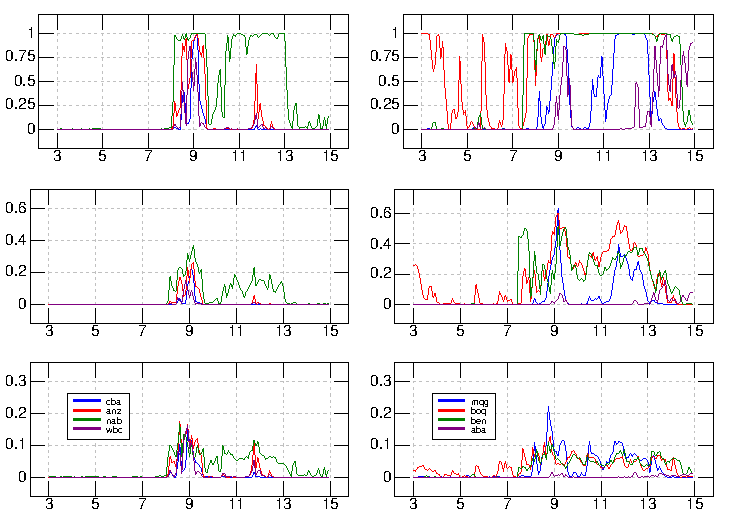
\includegraphics[width=12cm]{figures/default.pdf}
\caption{\br\ (top panels) and \pr\ (bottom panels) based on one month ahead  forecasts of $S^+$ for   major (left panel) and  minor (right panel)  Australian banks 2003--2014.  PRISK is based on worst monthly market outcome in 1 year.  Note different y--scale on top and bottom panels.}\label{default}
\end{center}
\end{figure}

\fref{sysstress} gives a picture of the relative magnitudes of \br\ and \pr\ in each of the eight banks.   For the major banks NAB stand out as, having \br\ more dominant than \pr\ and generally having heightened levels of \br.   ANZ appears to have relatively higher levels of \pr.    For the minors, MQG has persistently higher levels of \pr\ with BOQ and BEN comparable ratios and ABA having virtually no \pr\ compared to \br\ at any level of the latter. 

\begin{figure}[htbp]
\begin{center}
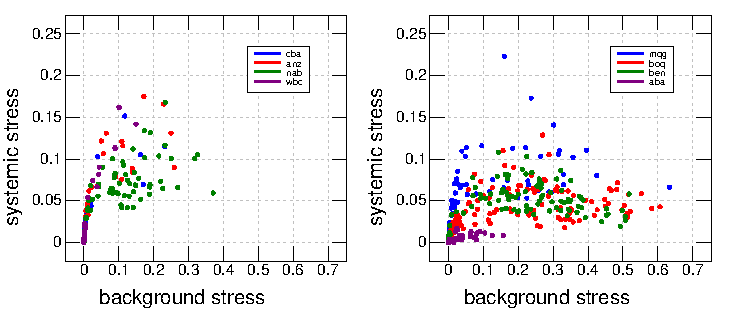
\includegraphics[width=12cm]{figures/sysstress.pdf}
\caption{\pr\  (y--axis) versus \br\  (x--axis)   for major  (left panel) and  minor banks (right panel)  for 144 months 2003--2014}
\label{sysstress}
\end{center}
\end{figure}


\section{Monitoring aggregate  stress}\label{aggregate}

\cite{brownlees2015} defines systemic risk in terms of $\Es(S)$. However $\Es(S)$ combines both baseline stress, due to high volatility or leverage, and the imposed system stress. To understand the nature of stress it is important to understand the mix of these two different stresses.

\subsection{Alternative aggregate stress measures}  

Two practical alternatives to SRISK for aggregating risk in financial institutions are set out \tref{aggstress}.  
The first row of the table reproduces the definition of SRISK in \eref{srisk} and decomposes \eref{srisk} into \br\ and \pr.  It is apparent that \sr\  measures a mix of \br\ and \pr.   Further heightened risk only arises if there is an ``on average"  shortfall.   Thus SRISK is relatively insensitive to tail events .

\begin{table}[htbp]
\caption{Measures of aggregate stress}\label{aggstress}
\small
\begin{center}
\begin{tabular}{l|l}
\hline
Measure&Expression\\
\hline
SRISK \citep{brownlees2015} & $\sum_i\{\Es(S_i)\}^+=\sum_i\{\br(S_i)+\pr(S_i)\}^+$ \\
No shortfall diversification: $S^*\equiv\sum_iS_i^+$  &$\sum_i\Es(S_i^+)=\br(S^*) +\pr(S^*)$ \\
Shortfall diversification:
$ S\equiv \sum_iS_i$&$\Es\{(\sum_iS_i)^+\}=\br(S^+) +\pr(S^+)$\\
\hline
\end{tabular}
\end{center}
\normalsize
\end{table}%

The second aggregation of risk displayed in \tref{aggstress} uses $S^*$, the  sum of positive shortfalls across firms.  With $S^*$, shortfall within a firm is not offset by averaging  nor with surpluses in other firms. The measure is thus more sensitive to tail risk.   A direct calculation shows 
\be{percc}
\frac{\Es(S_i^+)}{\Es(S^*)} =  \frac{\pr(S^+_i)}{\pr(S^*)}+\frac{\E(S^*)}{\Es(S^*)}\left\{\br_\%(S^+_i)-\pr_\%(S^+_i)\right\}\ .
\ee
The analyses in \sref{simulate1} suggest \br\ tends to dominate \pr.   Thus total risk tends to be dominated by \br.
 
 The final  row measure of \tref{aggstress}  allows for pooling of  shortfall across firms.  Since $S^*\ge S^+$ and both \br\  and \pr\ are additive 
 $$
 \sum_i\br(S_i^+)=\br(S^*)\ge\br(S^+)\ ,
 $$$$
 \sum_i\pr(S_i^+)=\pr(S^*) = \pr(S^+)+\pr(S^*-S^+)\ .
 $$
The difference $S^*-S^+$ is the ``diversifiable" shortfall and $\pr(S^*-S^+)$ measures the covariance between the diversifiable shortfall and  stress $\psi$.

System resilience aims to answer the question of whether the system as a whole can absorb shocks.   The capacity to absorb relies on implicit merging and hence on a measure of shortfall such as $S^+$.    When two firms merge the leverage of the resulting firm is less than that of the more highly leveraged firm.   The merged firm is more able to withstand return on equity shocks  unless negative shocks are more prone for the merged firm.   Similarly when many firms merge  puts $S^+$ for the conglomerate become less valuable.

Firms do not necessarily merge, even in dire financial circumstances.   Hence the mergers spoken of here are hypothetical.   From a regulators perspective, what would happen under a merger of all firms (or perhaps a group of firms) is nevertheless of interest.   A system as as a whole near Basel breach is more threatening that one where a few firms are near Basel breach but the system as a whole is strongly Basel compliant.

\subsection{Aggregate stress in the Australian banking sector}\label{monitoring}
 \tref{twodates} contains real time stress calculations on the first trading day of  January 2009 and December 2014.  As before there is no look ahead bias -- calculations on each of the two dates use data available on the first day of the applicable month.   The first eight rows in in the body of \tref{twodates} correspond to the eight banks used in this study.  The first  and second columns in the two halves of the table body contain the 
 Adjusted log--leverage  and debt  (as a percentage of total sustem debt) for each of the banks. 

\begin{table}[ht]
\caption{One month ahead bank stress projections}
\label{twodates}
\centering
\begin{threeparttable}
\small
\vspace{4mm}
\begin{tabular}{l|rrrr|rrrr}
\hline
&\multicolumn{4}{c|}{January 2009}&\multicolumn{4}{c}{December 2014}\\
  \hline
   & Aloglev& Debt & \br  & \pr  & Aloglev & Debt  &\br & \pr\\  
 %  & $\ell$ & $d$ &$\E(S_i^+)$&$\Psi(S_i^+)$& $\ell$&$d$ & $\E(S_i^+)$ & $\Psi(S_i^+)$ \\
  \hline
CBA & 18.57 & 24.30 & 22.99 & 29.60 & -70.34 & 22.70 & 0.00 & 0.00 \\ 
  ANZ & 15.93 & 18.37 & 14.87 & 18.89 & -38.64 & 22.10 & 0.00 & 0.00 \\ 
  NAB & 31.97 & 25.50 & 39.98 & 19.41 & -12.45 & 25.61 & 50.52 & 67.13 \\ 
  WBC & -1.55 & 22.84 & 5.86 & 23.94 & -53.84 & 22.03 & 0.00 & 0.00 \\ 
  MQG & 41.22 & 5.75 & 11.02 & 5.46 & -46.10 & 4.33 & 0.17 & 0.12 \\ 
  BOQ & 63.30 & 1.32 & 3.55 & 0.99 & -17.05 & 1.33 & 0.80 & 1.34 \\ 
  BEN & 18.91 & 1.81 & 1.72 & 1.71 & -7.63 & 1.84 & 25.43 & 30.71 \\ 
  ABA & -8.12 & 0.10 & 0.00 & 0.00 & 9.22 & 0.07 & 23.07 & 0.71 \\ 
  \hline
  Total $S^*$ & 18.78 & 2.42 & 17.17 & 8.63 & -41.91 & 3.27 & 0.03 & 0.12 \\ 
  Pooled $S^+$ & 17.81 & 2.42 & 15.28 & 10.18 & -44.22 & 3.27 & 0.00 & 0.00 \\ \hline
\end{tabular}
\begin{tablenotes}
\item[]The main body of table uses shortfall measure $S_i^+$. Aloglev is 100 times the adjusted log--leverage. \pr\  is with respect to expected worst monthly market return  in 12 months.  Main body of table displays percentage contributions of each firm to totals displayed in ``Total" row.   Total row displays 100 times debt weighted adjusted log--leverage, total debt in \$$10^{11}$, and \br\  and \pr\  per $0.08\times$debt and based on $S^*$.  Pooled row displays results with debt and equity pooled across banks and results based on $S^+$. 
\end{tablenotes}
\end{threeparttable}
\end{table}
\normalsize

January 2009 was a time of great stress for all eight banks.       Six of the eight banks were in Basel default with positive capital shortfalls as indicated by the adjusted log--leverage column:   the two banks not in Basel default were WBC and ABA.    
 
 Percentage \br\  and \pr\  are displayed in the next 2 columns in each half of the table.    The baseline stress column indicates most of the baseline stress arises from NAB -- almost 40\% of the total.   The next most baseline stressed bank is CBA with WBC also a substantial contributor.   The MQG bank contributes almost double to baseline stress compared to the proportion of total debt  it carries.  The other three small banks contribute relatively little to baseline stress with BOQ  almost 3 times expected on the basis of its debt.   \pr\   is highest for the CBA, higher than expected on the basis of its debt load and hence CBA was most susceptible to stress from additional general market equity devaluation.    All other banks appear have \pr\ comparable to their size in terms of debt load with only NAB being less systemically important.    This should be compared to NAB's high baseline stress.

Continuing with January 2009, the final two rows indicate the total amount of stress in the system and it's diversifiability.    
The second last  row labelled ``Total"  displays, in order, debt weighted adjusted log--leverage, total \br\  and total \pr.  On aggregate Total \br\  is about twice \pr.   Thus there is more danger of increasing capital shortfall due to market volatility  as opposed to further stress from further substantial general market devaluation.  The final row indicates stresses are not diversifiable:    The marginally  smaller  ``diversified"  baseline stress is offset by an increase in \pr.   

Stress readings  change dramatically when moving to December 2014 -- there is virtually no stress in any bank and the small amount of  stress in the system is diversifiable.    Most  \br\ is carried by NAB with lesser contributions by BEN and ABA.    All the stress in the minor bank ABA is baseline stress as only NAB and NAB have substantial \pr\  contributions.   Again, however, it must be emphasised that there is minimal systemic stress in the system.  Notice total debt in the banking sector  jumps about 35\% between the two dates.

The two  panels of \fref{fig6} track  \br\ and \pr\ for the banking sector as a whole through time.   There is virtually no risk in the system till late 2007 and the early warnings show a buildup in \br\ in $S^*$ compared to $S^+$.   Thus initially all \br\ is diversifiable suggesting \br\ is building up in a few banks.   This pattern of diversifiability in \br\ is generally maintained except at the peak of the crisis at the beginning of 2009 and in late 2011.  This pattern of \br\ buildup is evident in the bottom panel displaying all \br\ is, for small levels of risk initially absorbable -- that is present in $S^*$ but not present in $S^+$. 

The top right panel in \fref{fig6} displays the time series behaviour of \pr.  Generally \pr\ is less than \br.   Further, in situations of elevated risk,  \pr\ in $S^+$ exceeds that in $S^*$ indicating systemic stress from a general market downturn is greater in the system as a whole than its constituent parts.   Again, however, as displayed in the bottom right panel, \pr\ initially builds up in $S^*$, and only later manifests itself in $S^+$.  However the buildup is rapid so that with significant \pr\ the level in $S^+$ exceeds that in $S^*$.

\begin{figure}[htbp]
\begin{center}
 \begin{tabular}{cc}
      \resizebox{55mm}{!}{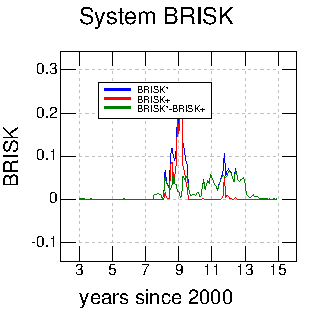
\includegraphics{figures/fig6a.pdf}} &
      \resizebox{55mm}{!}{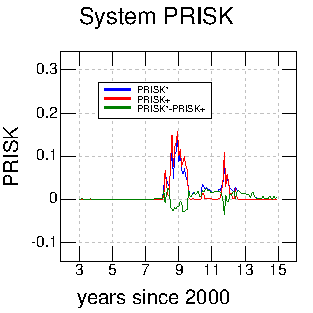
\includegraphics{figures/fig6b.pdf}}\\
    \end{tabular}
\caption{One month ahead system BRISK and PRISK based on predicted $S^*$ and $S^+$   from the beginning of 2003 through to end of 2014.}\label{fig6}
\end{center}
\end{figure}

%  Bottom panels  plot  two measures in the corresponding top 
% panel against each other: On the left \br($S^+$) on y--axis versus % \br($S^*$) on x--axis, and similarly for  \pr\ in the bottom right 
% panel.


\section{Risk weighted asset methodology}\label{riskmethod}

This section displays the application of the current stress framework to  the  risk weighting asset (RWA) methodology often used in determining capital shortfall.   RWA in effect assesses future stressed assets,   as opposed to, with SRISK,  future equity.   The same stress methodology can be used to stress assets.

Given debt $d$ and equity $w$ for a firm at a particular point of time,  assets are
$$
d+w=\sum_ja_j\ ,
$$
where $a_j$ denotes the value of assets in asset class $j$.   Future shortfall is, equivalent to \eref{fshortfall},  
\be{shortfall2}
S\equiv  d-(1-k)\sum_ja_j\e^{r_j}\ ,
\ee
where $r_j$ is the (uncertain) log--return on assets $a_j$.  With the risk weighting methodology the weights $a_j$  are replaced by $a_j/\sigma_j$ where $\sigma_j\ge 1$ is a ``risk" weight with large  weights assigned to  assets  with large perceived ``riskiness." 

Suppose $S$, $d$ and $r$ are the vectors of shortfalls, debts  and returns, respectively for the firms, and matrix $A$ has rows corresponding to the asset values of different firms.  Then the vector of firm shortfalls is
$$
S = d-(1-k)A\e^{r}\ ,
$$ 
where  exponentiation is componentwise.   Writing $S^+$ as the vector of positive shortfalls then, as in \sref{aggregate}, two aggregate measures of expected shortfall are $S^*\equiv \sum_iS_i^+$ and $(\sum_iS_i)^+$ where $S_i$ is component $i$ of vector $S$.

Estimation of \br\ and \pr\ can proceed via simulation:
$$
\omega\sim f(\omega)\cq r(\omega)\sim f(r|\omega)
$$
where $r(\omega)$ is  the simulated vector of returns for the asset classes given scenario $\omega$.   The vector of shortfalls corresponding to $\omega$ is then $S(\omega)=d-(1-k) A\e^{r(\omega)}$  where $A$ is the matrix with row $i$ corresponding to the current asset values for firm $i$ and $\e^{r(\omega)}$ denotes componentwise exponentiation.   Then the vectors of \br\ and \pr, with components corresponding to the different firms $i$ are estimated as  
\be{srisk4}
\br(S^+)\approx \frac{1}{N}\sum_\omega S^+(\omega)\cq
 \pr(S^+)\approx \frac{1}{N}\sum_\omega  \{\psi(\omega)-1\}S^+(\omega)\ ,
\ee
with similar results for $S^*=\sum_iS_i^+$ and $(\sum_iS_i)^+$.  

Stressful scenarios can be implicitly constructed via the following percentile method.   Suppose $r\sim f(r)$ are simulations from the joint distribution of future asset returns.   Returns for each asset class are  ranked yielding simulated percentile vectors $\omega$.   Denote $S(\omega)$ as the vector of shortfalls computed as before from returns $r$ corresponding to $\omega$.   Then use these $S(\omega)$  in the expressions \eref{srisk4} with
$$
\psi(\omega) = nc(\omega)\prod_j \{1-(1-\omega_j)^{n-1}\}\ ,
$$
where $c(\omega)$ is a copula density designed to exaggerate the juxtaposition of  adverse percentile occurrences: such as exaggerated lower tail dependence.   If $c(\omega)\equiv 1$  there is no exaggeration  and the copula associated with the $r(\omega)$ is the copula induced by $f(r)$.  If $n=1$ there is no sculpting of the marginal distributions.



\section{Conclusion}\label{conclude}

This paper presents a consistent methodology for stress testing and the measurement of  risk using the concept of stressed expectations.   Stressed expectation  formalises stress testing widely used in practice.  Stresses are introduced using a stress function and systemic stress uses a stress function based on system wide variables.   Methods and concepts are applied to publicly available time series of Australian bank data to monitor stress in Australian banks over time.   The methods identity banks in distress and those with high contribution to systemic stress.

\bigskip
\begin{center}
{\large\bf SUPPLEMENTARY MATERIAL}
\end{center}

\appendix
\renewcommand*{\thesection}{\Alph{section}}

\section{GARCH--DCC model}\label{garchdcc}

Denote the daily (log) return for firm $i$ at time $t$ as
\newcommand{\vareps}{\varepsilon}
\be{mean.model}
\delta_{it}=\mu_i+\sigma_{it}\eps_{it}\cq \eps_{it}\sim (0,1)\ .
\ee
The volatility $\sigma_{it}$ is modelled as
\be{vol}
\sigma_{i,t+1}^2 = \omega+ \sigma^2_{it}\{\beta+(\alpha+\gamma \eps^-_{it})\eps_{it}^2\}  \cq  \eps^-_{it}\equiv I(\eps_{it}<0)=I(\delta_{it}<\mu)\ ,
\ee
where $I$ denotes the indicator function.  Hence the response of $\sigma_{i,t+1}^2$ to $\eps_{it}^2$  is increased by $\gamma$   if
the rate of return is below the average $\mu_i$, compared to the response if $\delta_{it}>\mu_i$.  Equations \eref{mean.model} and \eref{vol} defined a simple threshold GARCH model:  called the TARCH(1,1).   In \eref{mean.model} the mean $\mu_i$ does not vary with time $t$ and in \eref{vol} it is assumed the terms  $\sigma_{it}^2$ and $\eps_{it}$ in the right hand side of \eref{vol} are sufficient to structure the dynamics of volatility and contemporaneous correlation.

The model defined by \eref{mean.model} and \eref{vol} is estimated  for each security $i$ jointly with  a similar model for  the market,  $i=m$.   Correlation between security $i$ and the market $m$ are implicitly modelled using  positive definite recursions   \citep{engle2002dynamic}
$$
(Q_{i,t+1}-S) = \alpha (\eta_{it}\eta_{it}'-S) + \beta (Q_{it}-S)\cq \eta_{it}\equiv(\eps_{it},\eps_{mt})' .
$$
The correlation defined by $Q_{it}$ is used as the correlation between $\eps_{it}$ and $\eps_{mt}$.


\section{Data sources}\label{data}

Data are sourced from DataStream using the company and datatype codes as set out in \tref{datastream}.

\begin{table}\caption{DataStream codes}\label{datastream}
\begin{center}
	\begin{tabular}{l|l}
	\hline
	\multicolumn{2}{l}{Company codes}\\
	\hline
A:ANZX & Australia and New Zealand Banking Group Limited\\
A:ABAX & Auswide Bank Limited\\
A:BOQX & Bank of Queensland Limited\\
A:BENX & Bendigo and Adelaide Bank Limited\\
A:CBAX & Commonwealth Bank of Australia\\
A:MQGX & Macquarie Bank Limited\\
A:NABX & National Australia Bank Limited\\
A:WBCX & Westpac Banking Corporation.\\
\hline
\multicolumn{2}{l}{Datatype codes}\\
\hline
	NOSH & Number of Shares\\
	P & Price\\
	WC02999 & Total Assets\\
	WC03501 & Shareholders Equity\\
	RZ & Total return index\\
\hline	
\end{tabular}
\end{center}
\end{table}

Firm equity $w$ is Number of Shares multiplied by Price. Firm debt $d$ is Total Assets minus Shareholders Equity. Stock returns are computed from the Total Return Index including paid dividends. 

\section{Computations}

All model fits in this paper are performed using the R language \citep{R-Development-Core-Team:2008aa} and in particular the rmgarch package described by \cite{ghalanos2012rmgarch}.  All other calculations including simulations are implemented in the J language \citep{iverson2003j}.

In the forward simulated forward projections the  innovations are chosen randomly from past innovations.   These past innovations are chosen consistently:  at a particular $t$ either all or none of $\eps_{it}$ are chosen.

\bibliography{piet2}
\end{document}
